\input templates/header
\title[ASD - Hashing]{\textbf{Algoritmi e Strutture Dati}\\[24pt]Hashing}

\usepackage{tikz}

\usepackage{listings}
\lstset{
  basicstyle=\ttfamily,
  columns=fullflexible,
  keywordstyle=\color{red}\bfseries,
  commentstyle=\color{blue},
  keepspaces=true,
  showstringspaces=false,
  tabsize=4,
  escapeinside={<@}{@>},
}


\graphicspath{{figs/07/}}

\begin{document}

%-------------------------------------------------------------------------
\FrameTitle{}

%-------------------------------------------------------------------------
\FrameContent

%%%%%%%%%%%%%%%%%%%%%%%%%%%%%%%%%%%%%%%%%%%%%%%%%%%%%%%%%%%%%%%%%%%%%%%%%%
\section{Introduzione}

\subsection{Motivazioni}

\begin{frame}[fragile]{Array associativi, mappe e dizionari}

\vspace{-12pt}
\begin{columns}[T]
\column{0.45\textwidth}
\begin{myboxtitle}[Python]
\vspace{-6pt}
\begin{lstlisting}[language=python]	
>>> v = {}
>>> v[10] = 5
>>> v["10"] = 42
>>> print(v[10]+v["10"])
<@\textcolor{blue}{47}@>
\end{lstlisting}
\end{myboxtitle}
\column{0.51\textwidth}
\begin{myboxtitle}[Go]
\vspace{-6pt}
\begin{lstlisting}	
ages := make(map[string]int)
ages["alice"]=45
ages["alberto"]=45
ages["alberto"]++
delete(ages, "alice")
\end{lstlisting}
\end{myboxtitle}
\end{columns}
\begin{myboxtitle}[Java]
\vspace{-6pt}
\begin{lstlisting}[language=java]	
Map<String, String> capoluoghi = new HashMap<>();
capoluoghi.put("Toscana", "Firenze");
capoluoghi.put("Lombardia", "Milano");
capoluoghi.put("Sardegna", "Cagliari");
\end{lstlisting}
\end{myboxtitle}



\end{frame}




%-------------------------------------------------------------------------
\begin{frame}{Introduzione}

\vspace{-6pt}
\begin{myboxtitle}[Ripasso]
Un dizionario è una struttura dati utilizzata per memorizzare insiemi dinamici
di \alert{coppie $\langle$ chiave, valore $\rangle$}
\BI
\item Le coppie sono indicizzate in base alla chiave
\item Il valore è un "dato satellite"
\EI
\end{myboxtitle}

\TwoCols{
  Operazioni:
	\BI
	\item $\dictlookup(\mathit{key}) \rightarrow \mathit{value}$
	\item $\dictinsert(\mathit{key},\mathit{value})$
	\item $\dictremove(\mathit{key})$
	\EI
}{
  Applicazioni:
	\BI
	\item Le tabelle dei simboli di un compilatore
	\item I dizionari di Python
	\item \ldots
	\EI 
}

\end{frame}

\begin{frame}{Possibili implementazioni}

{\footnotesize
\begin{tabular}{ | P{1.3cm} | P{1.7cm} | P{1.6cm} | P{1.6cm} | P{1.6cm} | P{1.6cm} |}
\hline
& \textbf{Array non ordinato} & 	\textbf{Array ordinato} & \textbf{Lista} & \textbf{Alberi RB} & \textbf{Implemen. ideale} \\\hline
$\dictinsert()$ & $O(1),O(n)$ & $O(n)$ & $O(1), O(n)$ & $O(\log n)$ & $O(1)$ \\\hline
$\dictlookup()$ & $O(n)$ & $O(\log n)$ &  $O(n)$ &  $O(\log n)$ &  $O(1)$\\\hline
$\dictremove()$ & $O(n)$ & $O(n)$ & $O(n)$ & $O(\log n)$ & $O(1)$\\\hline
\textbf{foreach} & $O(n)$ & $O(n)$ & $O(n)$ & $O(n)$ & $O(n)$\\\hline
\end{tabular}
}

\BB{Implementazione ideale: \alert{tabelle hash}}

\BI
\item Si sceglie una \alert{funzione hash} $h$ che mappa ogni chiave $k \in \cal U$\\ in un intero $h(k)$ 
\item La coppia chiave--valore $\langle k,v \rangle$ viene memorizzata in un vettore nella posizione $h(k)$
\item Questo vettore viene detto \alert{tabella hash}
\item Hash: From French \alert{hacher} (“to chop”), from Old French \alert{hache} (“axe”)
\EI

\end{frame}

\subsection{Definizioni base}

\begin{frame}{Tabelle hash -- Definizioni}

\vspace{-6pt}
\BI
\item L'insieme delle possibili chiavi è rappresentato \\dall'\alert{insieme universo} $\cal U$
di dimensione $u$
\item Il vettore $T[0 \ldots m-1]$ ha dimensione $m$
\item Una funzione hash è definita come
\(
h: {\cal U} \rightarrow \{ 0, 1, \ldots, m-1 \}
\)
\EI	
\begin{center}
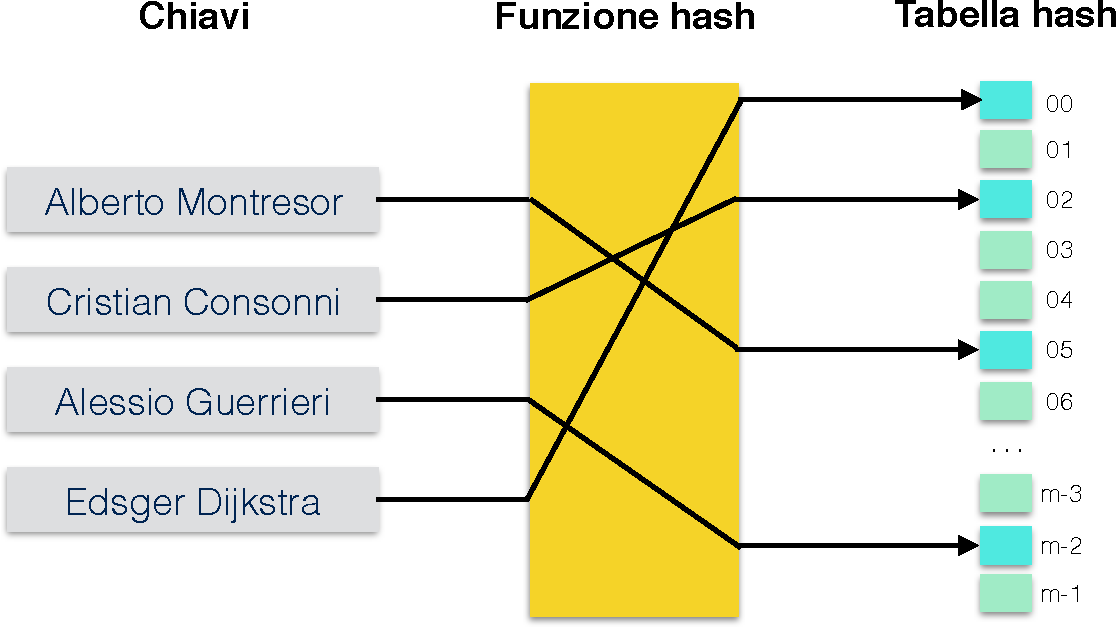
\includegraphics[width=0.7\textwidth]{hash-crop.pdf}
\end{center}

\end{frame}

\begin{frame}{Collisioni}

\vspace{-6pt}
\BI
\item Quando due o più chiavi nel dizionario hanno lo stesso valore hash, 
diciamo che è avvenuta una \alert{collisione}
\item Idealmente, vogliamo funzioni hash senza collisioni
\EI
\begin{center}
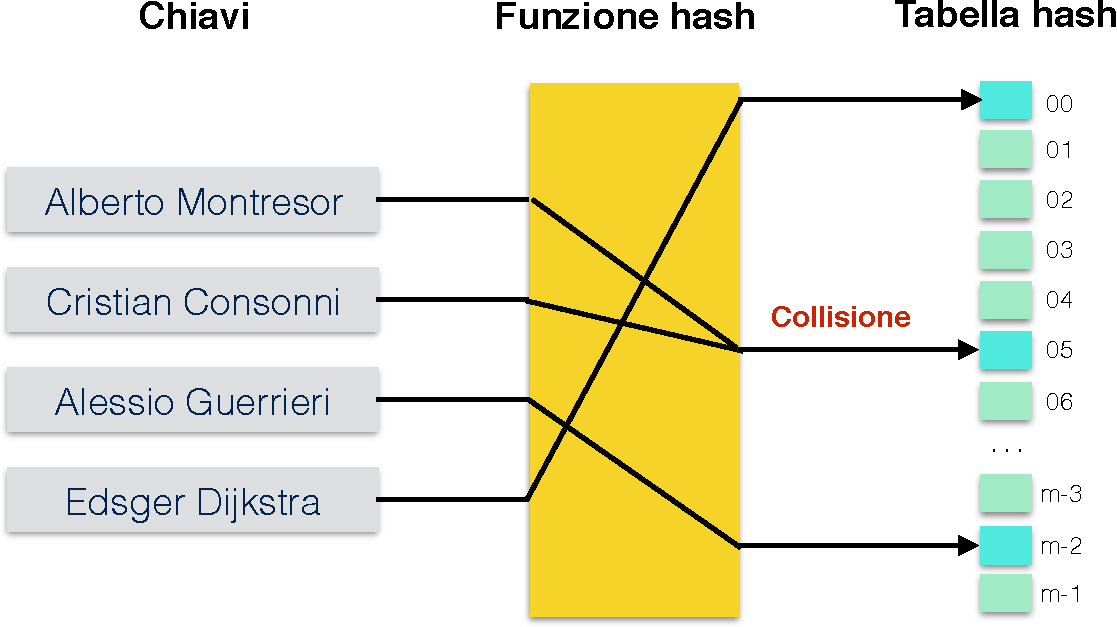
\includegraphics[width=0.7\textwidth]{collisioni-crop.pdf}
\end{center}

\end{frame}

\subsection{Tabelle ad accesso diretto}


\begin{frame}{Tabelle ad accesso diretto}

\vspace{-6pt}
\BB{Caso particolare: l'insieme ${\cal U}$ è già un sottoinsieme (piccolo) di $\mathbb{Z}^+$}
\begin{columns}[T]
\begin{column}{0.9\textwidth}
\BI
\item L'insieme dei giorni dell'anno, numerati da 1 a 366
\item L'insieme dei Pokemon di Kanto, numerati da 1 a 151
\EI
\end{column}
\begin{column}{0.1\textwidth}

\includegraphics[width=	\textwidth]{mewtwo.png}
\end{column}
\end{columns}

\begin{myboxtitle}[Tabella a accesso diretto]
\BI
\item Si utilizza la funzione hash identità $h(k)=k$
\item Si sceglie un valore $m$ pari a $u$
\EI
\end{myboxtitle}

\begin{myboxtitle}[Problemi]
\BI
\item Se $u$ è molto grande, l'approccio non è  praticabile 
\item Se $u$ non è grande ma il numero di chiavi 
effettivamentre registrate è molto minore di $u=m$, si spreca memoria
\EI
\end{myboxtitle}

\end{frame}

\section{Funzioni hash}

\subsection{Introduzione}

\begin{frame}{Funzioni hash perfette}

\vspace{-6pt}
\begin{myboxtitle}[Definizione]
Una funzione hash $h$ si dice \alert{perfetta} se è \alert{iniettiva}, ovvero
\[
\forall k_1, k_2 \in {\cal U}: k_1 \neq k_2 \Rightarrow h(k_1) \neq h(k_2)
\]
\end{myboxtitle}

\vspace{-9pt}
\begin{columns}[T]
\begin{column}{0.55\textwidth}
\BB{Esempi}
\BIL
\item Studenti ASD 2005-2016\\ N. matricola in $[100.090, 183.864]$\\[6pt]
\(
  h(k) = k - 100.090, m = 83.774
\)
\item Studenti immatricolati 2014\\ N. matricola in [173.185, 183.864]\\[6pt]
\(
h(k) = k - 173.185, m = 10.679
\)
\EIL
\end{column}
\hfill
\begin{column}{0.40\textwidth}
\BB{Problemi}
\BIL
\item Spazio delle chiavi spesso grande, sparso, non conosciuto
\item \EE spesso impraticabile ottenere una funzione hash perfetta
\EIL
\end{column}
\end{columns}

\end{frame}



\begin{frame}{Funzioni hash}

\vspace{-6pt}
\begin{myboxtitle}[Se non possiamo evitare le collisioni]
\BI
\item almeno cerchiamo di minimizzare il loro numero
\item vogliamo funzioni che distribuiscano \alert{uniformemente} le chiavi negli 
  indici $[0 \ldots m-1]$ della tabella hash
\EI
\end{myboxtitle}

\begin{myboxtitle}[Uniformità semplice]
\BI
\item Sia $P(k)$ la probabilità che una chiave $k$ sia inserita in tabella
\item Sia $Q(i)$ la probabilità che una chiave finisca nella cella $i$
\[
  Q(i) = \sum_{k \in {\cal U}: h(k)=i} P(k)
\]
\item Una funzione hash $h$ gode di \alert{uniformità semplice} se:
\[
  \forall i \in [0, \ldots, m-1] : Q(i) = 1/m
\]
\EI
\end{myboxtitle}

\end{frame}


\begin{frame}{Funzioni hash}

\vspace{-6pt}
\BB{\emph{Per poter ottenere una funzione hash con uniformità semplice,\\ la distribuzione delle probabilità $P$ deve essere nota}}

\begin{myboxtitle}[Esempio]
Se $\cal U$ è dato dai numeri reali in $[0,1[$  e ogni chiave ha la stessa probabilità di essere scelta, allora 
$H(k) = \lfloor km \rfloor$ soddisfa la proprietà di uniformità semplice
\end{myboxtitle}


\BB{Nella realtà}
\BIL
\item La distribuzione esatta può non essere (completamente) nota
\item Si utilizzano allora tecniche "\alert{euristiche}"
\EIL

\end{frame}

\subsection{Funzioni hash semplici}

\begin{frame}{Come realizzare una funzione hash}

\vspace{-6pt}
\begin{myboxtitle}[Assunzione]
Le chiavi possono essere tradotte in valori numerici non negativi, anche
interpretando la loro rappresentazione in memoria come un numero.
\end{myboxtitle}

\begin{myboxtitle}[Esempio: trasformazione stringhe]
\BI
\item $\mathit{ord}(c)$: valore ordinale binario del carattere $c$ in qualche codifica
\item $\mathit{bin}(k)$:	rappresentazione binaria della chiave $k$, concatenando i valori binari 
  dei caratteri che lo compongono
\item $\mathit{int}(b)$: valore numerico associato al numero binario $b$
\item $\mathit{int}(k) = \mathit{int}(\mathit{bin}(k))$
\EI
\end{myboxtitle}


\end{frame}

\begin{frame}{Come realizzare una funzion hash}

\vspace{-6pt}
\BB{Nei prossimi esempi}
\BIL
\item Utilizziamo codice ASCII a 8 bit
\EIL

\begin{align*}
\mathit{bin}("\texttt{DOG}") &= \makebox[2.1cm][l]{$\mathit{ord}("\mathtt{D}")$} \makebox[2.1cm][l]{$\mathit{ord}("\mathtt{O}")$} \makebox[2.1cm][l]{$\mathit{ord}("\mathtt{G}"$)} \\
	&= \makebox[2.1cm][l]{\texttt{01000100}} \makebox[2.1cm][l]{\texttt{01001111}} \makebox[2.1cm][l]{\texttt{01000111}} \\
\mathit{int}("\texttt{DOG}") &= \makebox[2.1cm][l]{$68 \cdot 256^2 + {}$} \makebox[2.1cm][l]{$79 \cdot 256 + {}$} \makebox[2.1cm][l]{$71$} \\
	&= 4,476,743
\end{align*}

\end{frame}

\begin{frame}{Funzione hash - Estrazione}

\vspace{-6pt}
\begin{myboxtitle}[Estrazione]
\BIL
\item $m = 2^p$
\item $H(k) = \mathit{int}(b)$, dove $b$ è un sottoinsieme di $p$ bit presi da $\mathit{bin}(k)$
\EIL
\end{myboxtitle}

\BB{Problemi}
\BIL
\item Selezionare bit presi dal suffisso della chiave può generare collissioni
con alta probabilità
\item Tuttavia, anche prendere parti diverse dal suffisso o dal prefisso può generare collisioni.
\EIL
 
\end{frame}

\begin{frame}{Funzione hash - Estrazione}

\vspace{-6pt}
\begin{myboxtitle}[Esempio 1]
$m = 2^p = 2^{16} = 65536$; $16$ bit meno significativi di $\mathit{bin}(k)$

\begin{align*}
\mathit{bin}("\texttt{Alberto}") = {} & \texttt{01000001  01101100  01100010  01100101} \\ 
&  \texttt{01110010  \alert{01110100  01101111}}\\
\mathit{bin}("\texttt{Roberto}") = {} & \texttt{01010010  01101111  01100010  01100101} \\
&    \texttt{01110010  \alert{01110100  01101111}} \\
H("\texttt{Alberto}") = {} & \mathit{int}(\alert{01110100  01101111}) = 29.807 \\
H("\texttt{Roberto}") = {} & \mathit{int}(\alert{01110100  01101111}) = 29.807
\end{align*}
\end{myboxtitle}


\end{frame}


\begin{frame}{Funzione hash - Estrazione}


\vspace{-6pt}
\begin{myboxtitle}[Esempio 2]
$m = 2^p = 2^{16} = 65536$; 16 bit presi all'interno di $\mathit{bin}(k)$

\begin{align*}
\mathit{bin}("\texttt{Alberto}") = {} & \texttt{0100\alert{0001  01101100  0110}0010  01100101} \\ 
&  \texttt{01110010  01110100  01101111}\\
\mathit{bin}("\texttt{Alessio}") = {} & \texttt{0100\alert{0001  01101100  0110}0101  01110011} \\ 
&  \texttt{01110011  01101001  01101111} \\
H("\texttt{Alberto}") = {} & \mathit{int}(\alert{0001011011000110}) = 5.830 \\
H("\texttt{Alessio}") = {} & \mathit{int}(\alert{0001011011000110}) = 5.830
\end{align*}
\end{myboxtitle}


\end{frame}

\begin{frame}[shrink=5]{Funzione hash - XOR}

\vspace{-6pt}
\begin{myboxtitle}[XOR]
\BIL
\item $m = 2^p$
\item $H(k) = \mathit{int}(b)$, dove $b$ è dato dalla somma modulo 2, effettuata bit a bit, di sottoinsiemi di $p$ bit di $\mathit{bin}(k)$
\EIL
\end{myboxtitle}

\BB{Problemi}
\BIL
\item Permutazioni (anagrammi) della stessa stringa possono generare lo stesso valore hash
\EIL


\end{frame}

\begin{frame}[shrink=5]{Funzione hash - XOR}

\vspace{-6pt}
\begin{myboxtitle}[Esempio]
$m = 2^{16} = 65536$; 5 gruppi di 16 bit ottenuti con 8 zeri di "\alert{padding}"

\begin{columns}[T]
\column{0.45\textwidth}
\begin{align*}
\mathit{bin}&("\texttt{montresor}") = \\ 
&\texttt{01101101 01101111}  \oplus {} \\
&\texttt{01101110 01110100} \oplus {} \\
&\texttt{01110010 01100101} \oplus {} \\
&\texttt{01110011 01101111} \oplus {} \\
&\texttt{01110010 \alert{00000000}} \\
H&("\texttt{montresor}") = {}\\
int&(\texttt{01110000 00010001}) = {}\\
& 28.689 
\end{align*}
\column{0.45\textwidth}
\begin{align*}
\mathit{bin}&("\texttt{sontremor}") = {} \\
&\texttt{01110011 01101111}  \oplus {} \\
&\texttt{01101110 01110100} \oplus {} \\
&\texttt{01110010 01100101} \oplus {} \\
&\texttt{01101101 01101111} \oplus {} \\
&\texttt{01110010 \alert{00000000}} \\
H&("\texttt{sontremor}") = {}\\
int&(\texttt{01110000 00010001}) = {}\\
& 28.689 
\end{align*}
\end{columns}

\end{myboxtitle}

\end{frame}


\begin{frame}{Funzione hash - Metodo della divisione}

\vspace{-6pt}
\begin{myboxtitle}[Metodo della divisione]
\BIL
\item $m$ dispari, meglio se numero primo
\item $H(k) = \mathit{int}(k) \bmod m$
\EIL
\end{myboxtitle}

\begin{myboxtitle}[Esempio]
$m = 383$
\begin{align*}
H("\texttt{Alberto}") =  &18.415.043.350.787.183 \bmod 383 =&  221 \\
H("\texttt{Alessio}") =  &18.415.056.470.632.815  \bmod 383 =& 77 \\
H("\texttt{Cristian}") = 4.8&60.062.892.481.405.294   \bmod 383 =& 130
\end{align*}

\end{myboxtitle}
   
\end{frame}


\begin{frame}{Funzione hash - Metodo della divisione}         

\vspace{-6pt}
\BB{Non vanno bene:}
\BIL
\item $m=2^p$: solo i $p$ bit meno significativi vengono considerati
\item $m=2^p-1$: permutazione di stringhe con set di caratteri di dimensione 
$2^p$ hanno lo stesso valore hash (Esercizio: dimostrare)
\EIL

\BB{Vanno bene:}
\BIL
\item Numeri primi, distanti da potenze di 2 (e di 10)
\EIL

\end{frame}

\begin{frame}{Funzione hash - Metodo della moltiplicazione (Knuth)}

\vspace{-6pt}
\begin{myboxtitle}[Metodo della moltiplicazione]
\BI
\item $m$ qualsiasi, meglio se potenza di $2$
\item $C$ costante reale, $0 < C < 1$
\item Sia $i = \mathit{int}(k)$
\item $H(k) = \left\lfloor m(C \cdot i - \lfloor C\cdot i \rfloor) \right\rfloor$
\EI
\end{myboxtitle}

\begin{myboxtitle}[Esempio]
\TwoColsCustom{0.15}{0.7}{
\medskip
$m = 2^{16}$\\ 
$C=\frac{\sqrt{5}-1}{2}$
}{
\smallskip
\begin{align*}
H("\texttt{Alberto}") = {} &65.536 \cdot 0.78732161432 = 51.598&   \\
H("\texttt{Alessio}") = {} &65.536 \cdot 0.51516739168 = 33.762&   \\
H("\texttt{Cristian}") = {} &65.536 \cdot 0.72143641000 = 47.280&   \\
\end{align*}
}
\end{myboxtitle}
   
\end{frame}

\begin{frame}{Metodo della moltiplicazione - Implementazione}


\vspace{-6pt}
\BIL
\item Si scelga un valore $m=2^p$
\item Sia $w$ la dimensione in bit della parola di memoria: $i, m \leq 2^w$
\item Sia $s = \lfloor C \cdot 2^w \rfloor$
\item $i \cdot s$ può essere scritto come $r_1 \cdot 2^w + r_0$
	\BI	
	\item $r_1$ contiene la parte intera di $iC$
	\item $r_0$ contiene la parte frazionaria di $iC$
	\EI
\item Si restituiscano i $p$-bit\\ più significativi di $r_0$
\EIL

\begin{tikzpicture}[remember picture,overlay]
    \node[xshift=-4.0cm,yshift=-7.2cm] at (current page.north east){%
		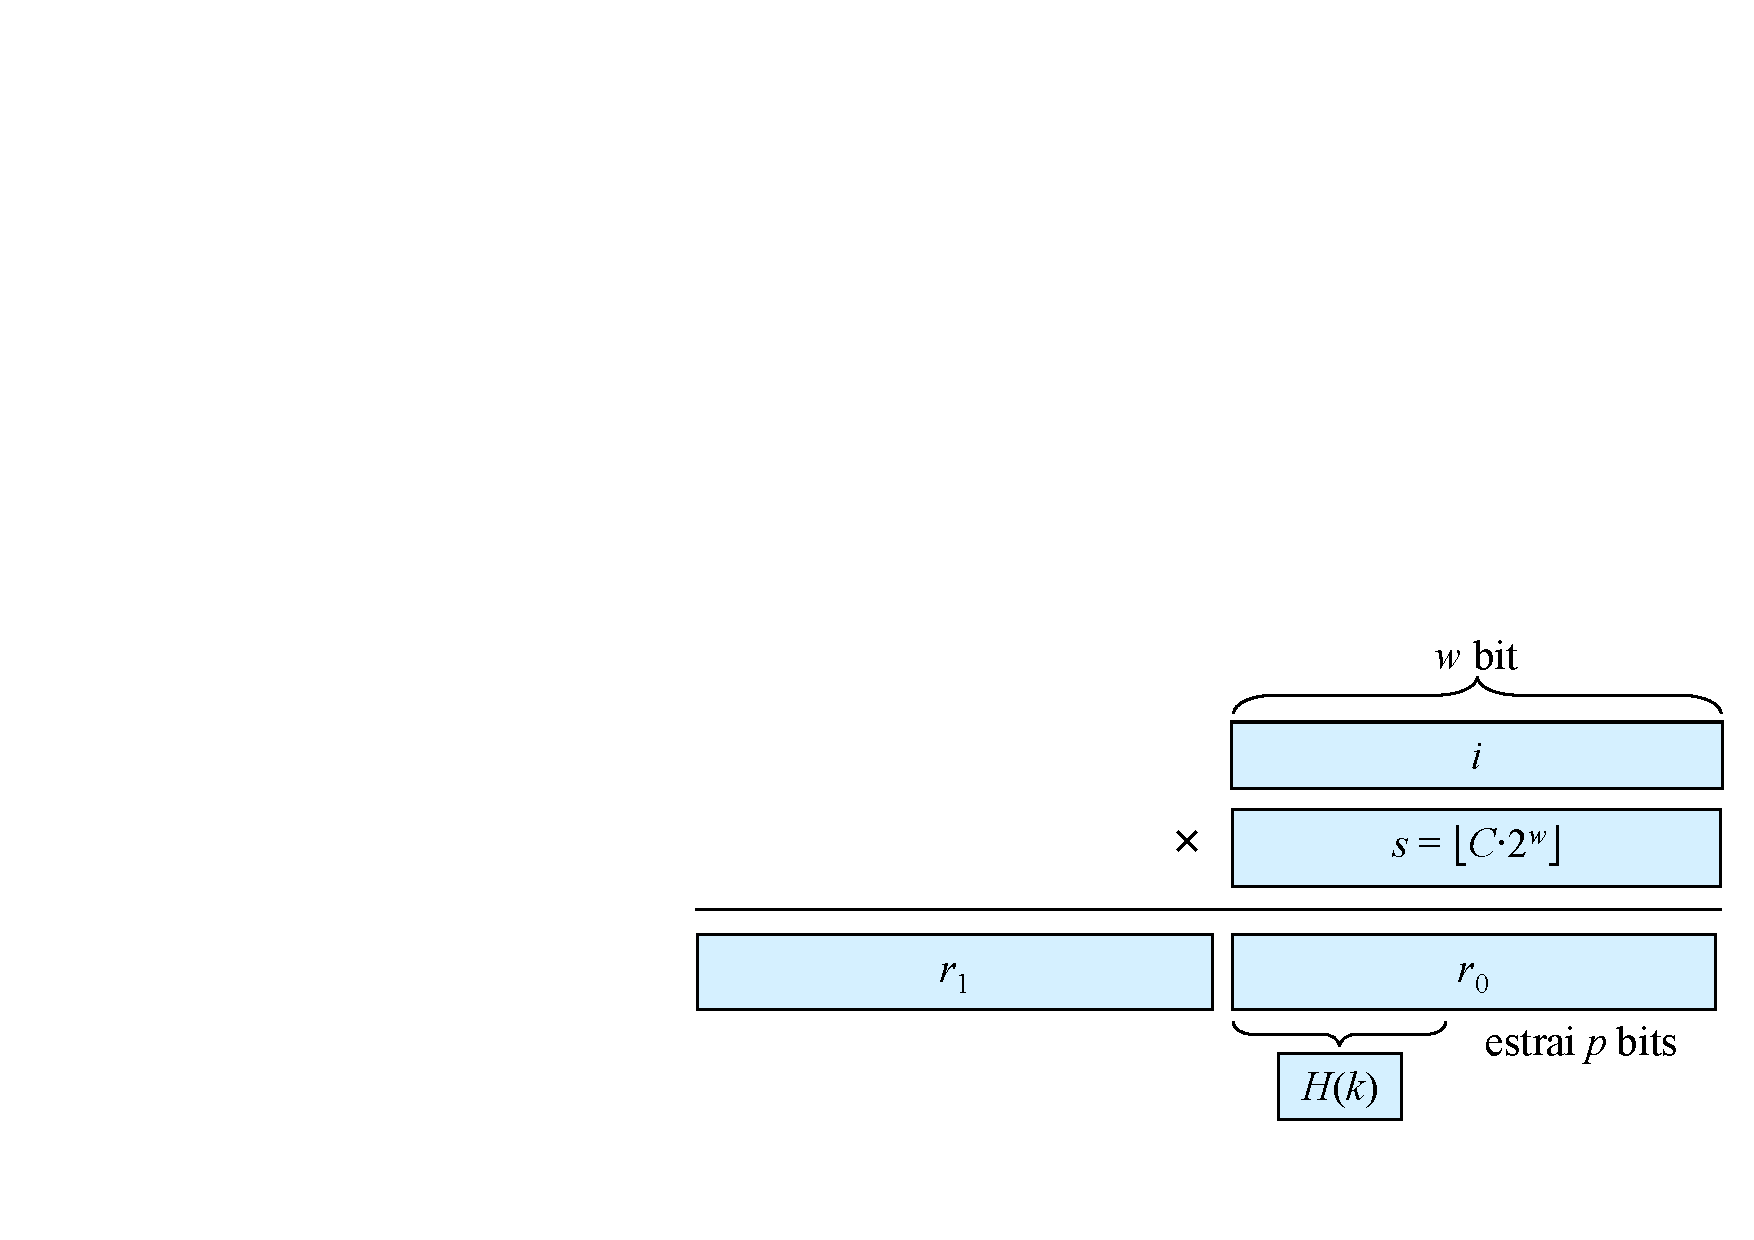
\includegraphics[width=7cm]{moltiplicazione.pdf}};
\end{tikzpicture}


\end{frame}

\subsection{Reality check}

\begin{frame}{Reality check}

\vspace{-6pt}
\BIL
\item Non è poi così semplice...
\BI
\item Il metodo della moltiplicazione suggerito da Knuth non fornisce hashing uniforme
\EI
\item  Test moderni per valutare la bontà delle funzioni hash
\BI
\item \alert{Avalanche effect}: Se si cambia un bit nella chiave, deve cambiare almeno la metà dei bit del valore hash
\item Test statistici (\alert{Chi-square})
\EI

\item Funzioni crittografiche (SHA-1)
\BI
\item Deve essere molto difficile o quasi impossibile risalire al testo che ha portato ad un dato hash;
\EI
\EIL

\end{frame}

\begin{frame}{Funzioni hash moderne}
	
{\renewcommand*{\arraystretch}{1.3}
\begin{tabular}{|P{2.5cm}|P{6cm}|P{2cm}|}
\hline
\textbf{Nome} & \textbf{Note} & \textbf{Link}
\\ \hline
FNV Hash & 
Funzione hash non crittografica, creata nel 1991.
&
[\href{https://en.wikipedia.org/wiki/Fowler-Noll-Vo_hash_function}{\alert{\underline{Wikipedia}}}]
[\href{http://isthe.com/chongo/tech/comp/fnv/}{\alert{\underline{Codice}}}]
\\ \hline
Murmur Hash &
Funzione hash non crittografica, creata nel 2008, il cui uso è ormai sconsigliato
perchè debole.
&
[\href{https://en.wikipedia.org/wiki/MurmurHash}{\alert{\underline{Wikipedia}}}]
[\href{https://github.com/aappleby/smhasher/}{\alert{\underline{Codice}}}]
\\ \hline
City Hash &
Una famiglia di funzioni hash non-crittografiche, progettate
da Google per essere molto veloce. Ha varianti a 32, 64, 128, 256 bit.
&
[\href{https://en.wikipedia.org/wiki/CityHash}{\alert{\underline{Wikipedia}}}]
[\href{https://github.com/google/cityhash/}{\alert{\underline{Codice}}}]
\\ \hline
Farm Hash &
Il successore di City Hash, sempre sviluppato da Google.
&
[\href{https://github.com/google/farmhash/}{\alert{\underline{Codice}}}]
\\ \hline
\end{tabular}
}
\end{frame}


\section{Gestione collisioni}


\begin{frame}{Problema delle collisioni}
	
\vspace{-6pt}
\BB{Come gestire le collisioni?}
\BI
\item Dobbiamo trovare posizioni alternative per le chiavi
\item Se una chiave non si trova nella posizione attesa, bisogna cercarla nelle posizioni alternative
\item Questa ricerca:
  \BI
	\item dovrebbe costare $O(1)$ nel caso medio
	\item può costare $O(n)$ nel caso pessimo
	\EI
\EI

\BB{Due possibili tecniche}
\BI
\item \alert{Liste di trabocco} o memorizzazione esterna
\item \alert{Indirizzamento aperto} o memorizzazione interna
\EI

\end{frame}

\subsection{Liste/vettori di trabocco}

\begin{frame}{Liste/vettori di trabocco (Concatenamento o Chaining)}

\vspace{-12pt}
\TwoColsCustom{0.48}{0.50}{
\BB{Idea}
\BIL
\item Le chiavi con lo stesso valore hash $h$ vengono memorizzate in una \alert{lista monodirezionale} / \alert{vettore dinamico}
\item Si memorizza un puntatore alla testa della lista / al vettore nello slot $H(k)$-esimo della tabella hash
\EIL
}{
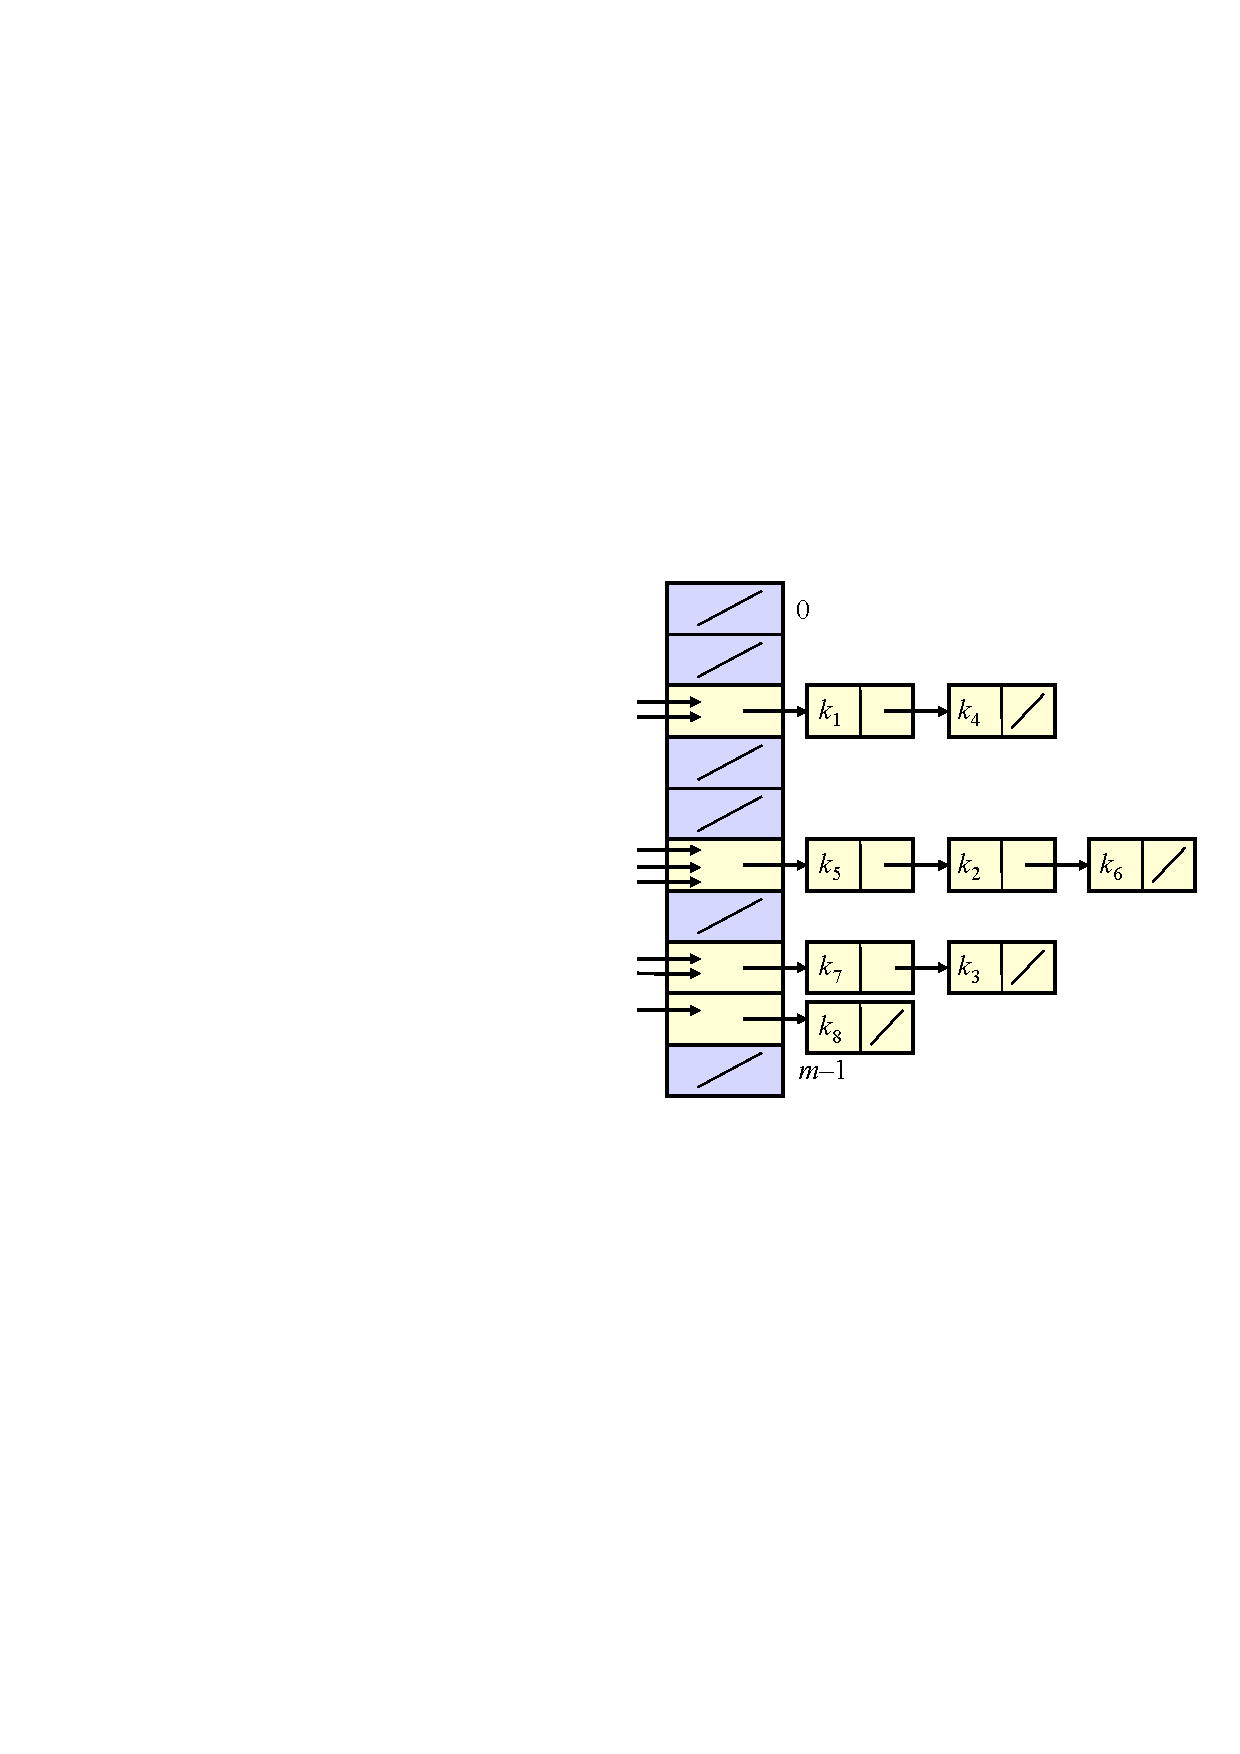
\includegraphics[width=1.0\textwidth]{trabocco.pdf}
}
	
\end{frame}

\begin{frame}{Liste/vettori di trabocco (Concatenamento o Chaining)}
\vspace{-12pt}
\TwoColsCustom{0.48}{0.50}{
\BB{Operazioni}
\BIL
\item \alert{\dictinsert()}:\\ inserimento in testa
\item \alert{\dictlookup()}, \alert{\dictremove()}:\\ 
scansione della lista per cercare la chiave
\EIL
}{
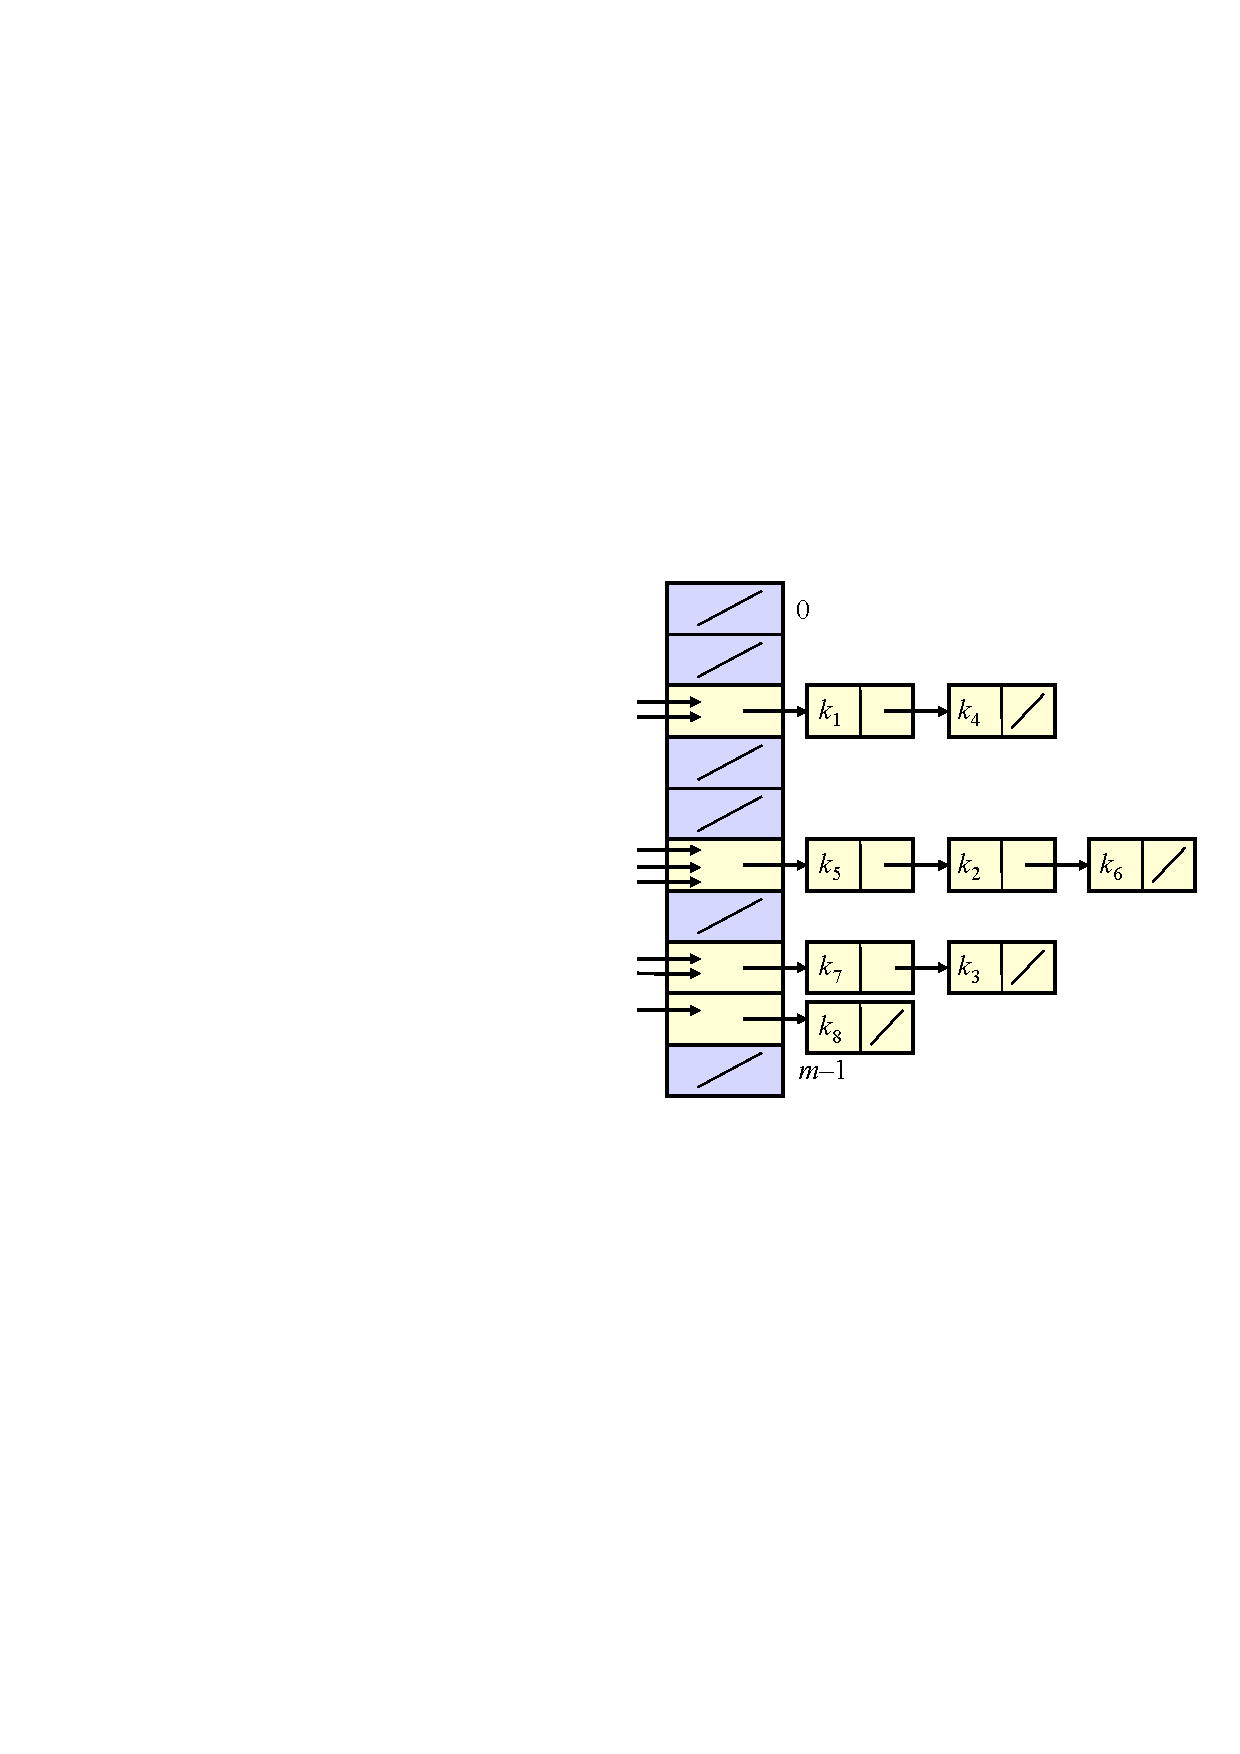
\includegraphics[width=1.0\textwidth]{trabocco.pdf}
}
	
\end{frame}


\begin{frame}{Liste/vettori di trabocco: analisi complessità}
	
{\renewcommand*{\arraystretch}{1.3}
\begin{tabular}{|P{1.7cm}|P{9.5cm}|}
\hline
$n$ & Numero di chiavi memorizzati in tabella hash \\ \hline
$m$ & Capacità della tabella hash \\ \hline
$\alpha = n/m$ & Fattore di carico \\ \hline
$I(\alpha)$ & Numero medio di accessi alla tabella per
la ricerca di una chiave non presente nella tabella (\alert{ricerca con insuccesso}) \\ \hline
$S(\alpha)$ & Numero medio di accessi alla tabella per
la ricerca di una chiave presente nella tabella 
(\alert{ricerca con successo}) \\ \hline
\end{tabular}
}

\BB{Analisi del caso pessimo}
\pause
\BI
\item Tutte le chiavi sono collocate in unica lista
\item \alert{\dictinsert()}: $\Theta(1)$
\item \alert{\dictlookup()}, \alert{\dictremove()}: $\Theta(n)$
\EI
	
\end{frame}

\begin{frame}{Liste/vettori di trabocco: analisi complessità}

\vspace{-6pt}
\BB{Analisi del caso medio: assunzioni}
\BIL
\item Dipende da come le chiavi vengono distribuite
\item Assumiamo hashing uniforme semplice
\item Costo calcolo funzione di hashing: $\Theta(1)$
\EIL

\BB{Quanto sono lunghe le liste / i vettori?}
\pause
\TwoCols{
\BIL
\item Il valore \alert{atteso} della lunghezza di
una lista è pari a $\alpha = n/m$
\EIL
}{
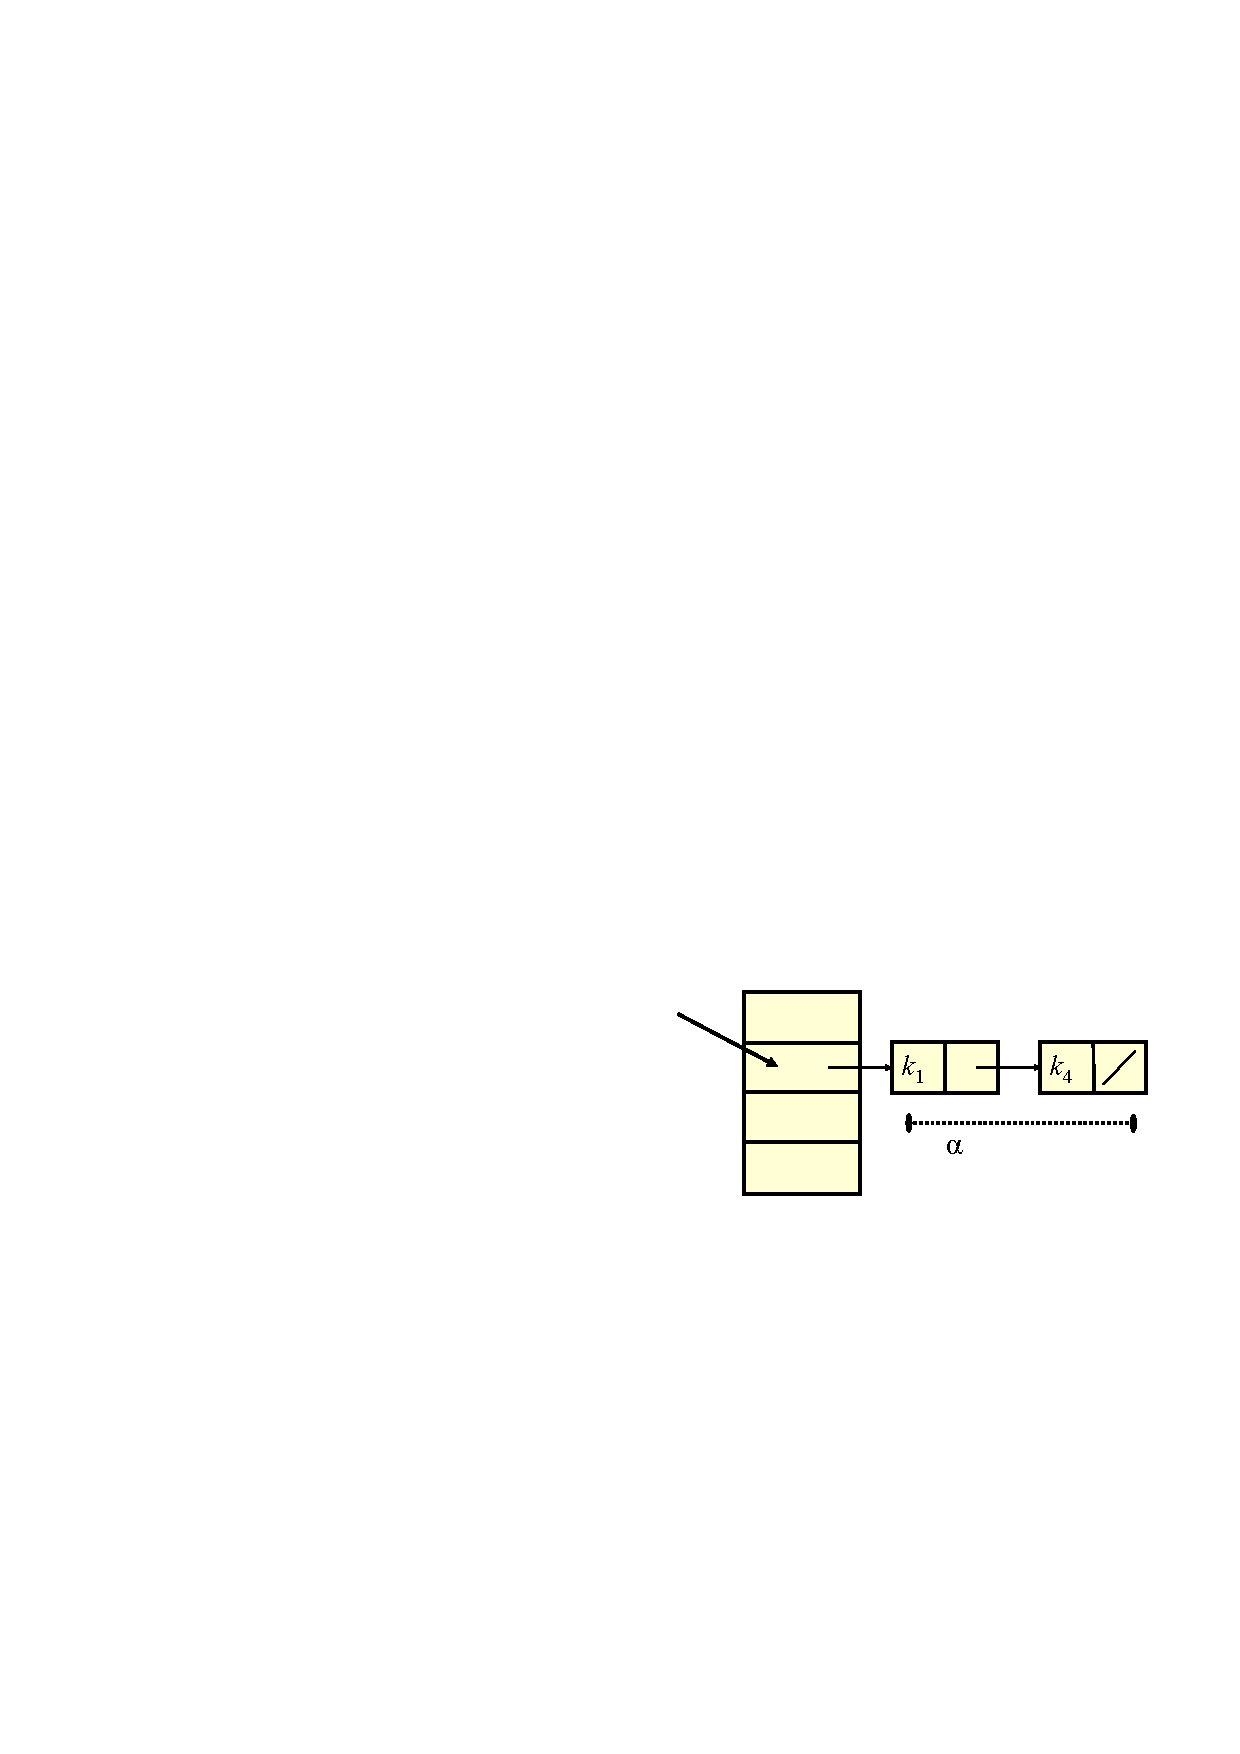
\includegraphics[width=\textwidth]{trabocco-alfa.pdf}
}

\end{frame}

\begin{frame}{Liste/vettori di trabocco: analisi complessità}

\vspace{-6pt}
\BB{Costo hashing}
\BIL
\item Una chiave \alert{presente} o \alert{non presente} in tabella può essere 
collocata in uno qualsiasi degli $m$ slot
\item Costo di hashing: $\Theta(1)$
\EIL

\vspace{-9pt}
\TwoCols{
\BB{Ricerca senza successo}
\BIL
\item Una ricerca \alert{senza successo} tocca tutte le chiavi nella lista corrispondente
\EIL
}{
\BB{Ricerca con successo}
\BIL
\item Una ricerca con \alert{successo} tocca in media metà delle chiavi nella lista corrispondente
\EIL
}

\pause
\smallskip
\TwoCols{
\BI
\item Costo atteso: \alert{$\Theta(1) + \alpha$}
\EI
}{
\BI
\item Costo atteso: \alert{$\Theta(1) + \alpha/2$}
\EI
}

\end{frame}

\begin{frame}{Liste/vettori di trabocco: analisi complessità}

\vspace{-6pt}
\BB{Qual è il significato del fattore di carico?}	
\BIL
\item Influenza il costo computazionale delle operazioni sulle tabelle hash
\item Se $n = O(m)$, $\alpha = O(1)$
\item Quindi tutte le operazioni sono $O(1)$
\EIL

\end{frame}

\subsection{Indirizzamento aperto}

\begin{frame}{Indirizzamento aperto}

\vspace{-6pt}
\BB{Problemi delle liste/vettori di trabocco}
\BIL
\item Struttura dati complessa, con liste, puntatori, etc.
\EIL

\smallskip
\BB{Gestione alternativa: \alert{indirizzamento aperto}}
\BIL
\item Idea: memorizzare tutte le chiavi nella tabella stessa
\item Ogni slot contiene una chiave oppure \Nil
\EIL

\vspace{-6pt}
\TwoColsCustom{0.45}{0.52}{
\BB{Inserimento}
Se lo slot prescelto è utilizzato, si cerca uno slot "alternativo"
}{
\BB{Ricerca}
Si cerca nello slot prescelto, e poi negli slot "alternativi" fino a quando non si trova la chiave oppure \Nil
}
\end{frame}

\begin{frame}{Definizioni}
\vspace{-6pt}
\begin{myboxtitle}[Ispezione]
Un'\alert{ispezione} è l'esame di uno slot durante la ricerca.
\end{myboxtitle}

\begin{myboxtitle}[Funzione hash]
\medskip
\TwoColsCustom{0.3}{0.60}{
Estesa nel modo seguente:
}{ 
\[
  H : {\cal U} \times \overbrace{[0 \ldots m-1]}^{\textrm{Numero ispezione}} \rightarrow \overbrace{[0 \ldots m-1]}^{\textrm{Indice vettore}}
\]
}
\end{myboxtitle}


\begin{myboxtitle}[Sequenza di ispezione]
Una \alert{sequenza di ispezione} $[ H(k, 0), H(k, 1), \ldots, H(k, m-1) ]$ è 
una \alert{permutazione} degli indici $[0, \ldots, m-1]$ corrispondente all'ordine
in cui vengono esaminati gli slot.
\BI
\item Non vogliamo esaminare ogni slot più di una volta	
\item Potrebbe essere necessario esaminare tutti gli slot nella tabella
\EI
\end{myboxtitle}
	
\end{frame}

\begin{frame}{Esempio}


\begin{overprint}
\includegraphics<1|handouts:0>[width=\textwidth,page=1]{ind-aperto.pdf}
\includegraphics<2|handouts:0>[width=\textwidth,page=2]{ind-aperto.pdf}
\includegraphics<3|handouts:0>[width=\textwidth,page=3]{ind-aperto.pdf}
\includegraphics<4|handouts:0>[width=\textwidth,page=4]{ind-aperto.pdf}
\includegraphics<5|handouts:0>[width=\textwidth,page=5]{ind-aperto.pdf}
\includegraphics<6|handouts:1>[width=\textwidth,page=6]{ind-aperto.pdf}
\end{overprint}

\end{frame}

\begin{frame}{Fattore di carico}

\vspace{-6pt}
\BB{Cosa succede al fattore di carico $\alpha$?}
\BIL
\item Compreso fra 0 e 1
\item La tabella può andare in overflow
\EIL


\end{frame}

\begin{frame}{Tecniche di ispezione}

\vspace{-6pt}
\begin{myboxtitle}[Hashing uniforme]
La situazione ideale prende il nome di \alert{hashing uniforme}, in cui
ogni chiave ha la stessa probabilità di avere come sequenza di ispezione
una qualsiasi delle $m!$ permutazioni di $[0, \ldots, m-1]$.
\end{myboxtitle}

\BIL
\item Generalizzazione dell'hashing uniforme semplice
\item Nella realtà:
\BI
\item E' difficile implementare il vero hashing uniforme
\item Ci si accontenta di ottenere almeno una permutazione
\EI
\item Tecniche diffuse:
\BI
\item \alert{Ispezione lineare}
\item \alert{Ispezione quadratica}
\item \alert{Doppio hashing}
\EI
\EIL

\end{frame}

\begin{frame}{Ispezione lineare}
	
\vspace{-6pt}
\BB{
Funzione: \alert{$H(k, i) = (H_1(k) + h \cdot i) \bmod m$}
}

\BIL
\item La sequenza $H_1(k)$, $H_1(k)+h$, $H_1(k)+2 \cdot h$, $\ldots$, $H_1(k)+(m-1) \cdot h$ 
(modulo $m$) è determinata dal primo elemento
\item Al massimo $m$ sequenze di ispezione distinte sono possibili
\EIL

\begin{myboxtitle}[\alert{Agglomerazione primaria} (primary clustering)]
\BI
\item Lunghe sotto-sequenze occupate...
\item ... che tendono a diventare più lunghe: uno slot vuoto preceduto da $i$ 
slot pieni viene riempito con probabilità $(i+1)/m$
\item I tempi medi di inserimento e cancellazione crescono	
\EI
\end{myboxtitle}
\end{frame}

\begin{frame}{Agglomerazione primaria}

\vspace{-6pt}
\begin{myboxtitle}[\alert{Agglomerazione primaria} (primary clustering)]
\BI
\item Lunghe sotto-sequenze occupate...
\item ... che tendono a diventare più lunghe: uno slot vuoto preceduto da $i$ 
slot pieni viene riempito con probabilità $(i+1)/m$
\item I tempi medi di inserimento e cancellazione crescono	
\EI
\end{myboxtitle}

\begin{overprint}
\includegraphics<1|handout:1>[width=\textwidth,page=1]{agglomerazione.pdf}
\includegraphics<2|handout:2>[width=\textwidth,page=2]{agglomerazione.pdf}
\includegraphics<3|handout:3>[width=\textwidth,page=3]{agglomerazione.pdf}
\includegraphics<4|handout:4>[width=\textwidth,page=4]{agglomerazione.pdf}
\includegraphics<5|handout:5>[width=\textwidth,page=5]{agglomerazione.pdf}
\end{overprint}

\end{frame}

\begin{frame}{Ispezione quadratica}
	
\vspace{-6pt}
\BB{
Funzione: \alert{$H(k, i) = (H_1(k) + h \cdot i^2) \bmod m$}
}

\BIL
\item Dopo il primo elemento $H_1(k,0)$, le ispezioni successive hanno un 
offset che dipende da una funzione quadratica nel numero di ispezione $i$
\item La sequenza risultante \alert{non è una permutazione}!
\item Al massimo $m$ sequenze di ispezione distinte sono possibili
\EIL

\begin{myboxtitle}[\alert{Agglomerazione secondaria} (secondary clustering)]
\BI
\item Se due chiavi hanno la stessa ispezione iniziale, le loro sequenze sono identiche
\EI
\end{myboxtitle}
\end{frame}


\begin{frame}{Doppio hashing}
	
\vspace{-6pt}
\BB{
Funzione: \alert{$H(k, i) = (H_1(k) + i \cdot H_2(k)) \bmod m$}
}

\BIL
\item Due funzioni ausiliarie:
\BI
\item $H_1$ fornisce la prima ispezione
\item $H_2$ fornisce l'offset delle successive ispezioni
\EI
\item Al massimo $m^2$ sequenze di ispezione distinte sono possibili
\item Per garantire una permutazione completa, $H_2(k)$ deve essere relativamente primo con $m$
\BI
\item Scegliere $m = 2^p$  e  $H_2(k)$ deve restituire numeri dispari
\item Scegliere $m$ primo, e $H_2(k)$ deve restituire numeri minori di $m$
\EI 
\EIL

\end{frame}


\begin{frame}{Cancellazione}

\vspace{-3pt}
\begin{overprint}
\onslide<1-2|handout:1-2>
	\BB{
		Non possiamo semplicemente sostituire la chiave che vogliamo cancellare con un $\Nil$. Perché?
	}
\onslide<3|handout:3>
	\BB{Approccio}
	\BI
	\item Utilizziamo un speciale valore \textbf{deleted} al posto di $\Nil$ per marcare uno 
			slot come vuoto dopo la cancellazione
		\BI
		\item Ricerca: 		\textbf{deleted} trattati come slot pieni
		\item Inserimento: 	\textbf{deleted} trattati come slot vuoti
		\EI
	\item Svantaggio: il tempo di ricerca non dipende più da $\alpha$
	\item Concatenamento più comune se si ammettono cancellazioni
\EI
\end{overprint}
\begin{overprint}
\includegraphics<2|handout:2>[width=\textwidth,page=1]{cancellazione.pdf}
\includegraphics<3|handout:3>[width=\textwidth,page=2]{cancellazione.pdf}
\end{overprint}
\end{frame}

\begin{frame}{Implementazione - Hashing doppio}

\RestyleAlgo{plain}

\vspace{-12pt}
\begin{Procedure}
\noindent\rule{\textwidth}{0.8pt}\hrulefill

\vspace{-3pt}
{\Hash}

\vspace{-9pt}
\noindent\rule{\textwidth}{0.8pt}\hrulefill

$\Item[\,]\ K$\REMR{Tabella delle chiavi}
$\Item[\,]\ V$\REMR{Tabella dei valori}
\INTEGER $m$\REMR{Dimensione della tabella}
\BlankLine

\PROCEDURE{\Hash \hashconstructor(\INTEGER $\hashsize$)}
{
  $\Hash\ t = \NEW\ \Hash$\;
  $t.m = \hashsize$\;
  $t.K = \NEW\ Item[0 \mldots \hashsize-1]$\;
  $t.V = \NEW\ Item[0 \mldots \hashsize-1]$\;
  \For{$i = 0$\ \TO\ $\hashsize-1$}{ $t.K[i] = \hempty$}
  \Return $t$\;
}
\BlankLine

\end{Procedure}
\end{frame}
 
\begin{frame}{Implementazione - Hashing doppio}
\vspace{-12pt}
\RestyleAlgo{plain}
\begin{Procedure}
\INTEGER\ \PROCEDURE{\hashscan(\Item $k$, \BOOLEAN \hinsert)}
{
  \INTEGER\ $c = m$\REMR{Prima posizione \emph{\hcancel}}
  \INTEGER\ $i = 0$\REMR{Numero di ispezione}
  \INTEGER\ $j = H(k)$\REMR{Posizione attuale}
  \While{$K[j] \neq k$ \AND\ $K[j] \neq \hempty$ \AND\ $i<m$}
  {
    \If{$K[j] \Eq \hcancel$ \AND\ $c\Eq m$}{$c = j$}
    $j = (j + H'(k)) \bmod m$\;
    $i = i+1$\; 
  }
  \If{$\hinsert$ \AND\ $K[j] \neq k$ \AND $c < m$}{$j = c$\;}
  \Return\ $j$\;
}
\BlankLine

\end{Procedure}
\end{frame}
 
\begin{frame}{Implementazione - Hashing doppio}
\vspace{-12pt}
\RestyleAlgo{plain}
\begin{Procedure}

\Item\ \PROCEDURE{\dictlookup(\Item $k$)}
{
  $\INTEGER\ i = \hashscan(k, \FALSE)$\;
  \eIf{$K[i] \Eq k$}{\Return\ $V[i]$\;}{\Return\ $\hempty$\;}
}
\BlankLine

\PROCEDURE{\dictinsert(\Item $k$, \Item $v$)}
{
  $\INTEGER\ i = \hashscan(k, \TRUE)$\;
  \eIf{$K[i] \Eq \hempty$ \OR\ $K[i] \Eq \hcancel$ \OR\ $K[i] \Eq k$}
  {
    $K[i] = k$\;
    $V[i] = v$\;
  }
  {
    \% Errore: tabella hash piena
  }
}
\end{Procedure}
\end{frame}
 
\begin{frame}{Implementazione - Hashing doppio}
\RestyleAlgo{plain}
\vspace{-12pt}
\begin{Procedure}

\PROCEDURE{\dictremove(\Item $k$)}
{
  $\INTEGER\ i = \hashscan(k, \FALSE)$\;
  \If{$K[i] \Eq k$}
  {
    $K[i] = \hcancel$\;
  }  
}
\end{Procedure}
\noindent\rule{\textwidth}{0.8pt}\hrulefill


\end{frame}


\begin{frame}{Complessità}

\begin{center}
\begin{tabular}{lccc}
\textbf{Metodo} & $\alpha$ & $I(\alpha)$ & $S(\alpha)$\\
\hline
Lineare & $0 \le \alpha < 1$ &
\parbox{2.8cm}{\[\frac{(1-\alpha)^2+1}{2(1-\alpha)^2}\]} &
\parbox{2.8cm}{\[\frac{1-\alpha/2}{1-\alpha}\]}\\
\parbox{3cm}{Hashing doppio}
& $0 \le \alpha < 1$ &
\parbox{2.8cm}{\[\frac{1}{1-\alpha}\]} &
\parbox{2.8cm}{\[-\frac{1}{\alpha}\ln (1-\alpha)\]}\\[7mm]
Liste di trabocco & $\alpha\ge 0$ & $1 + \alpha$ & $1 + \alpha/2$\\
\hline
\end{tabular}
\end{center}

\end{frame}	

\begin{frame}{Complessità}
	
	
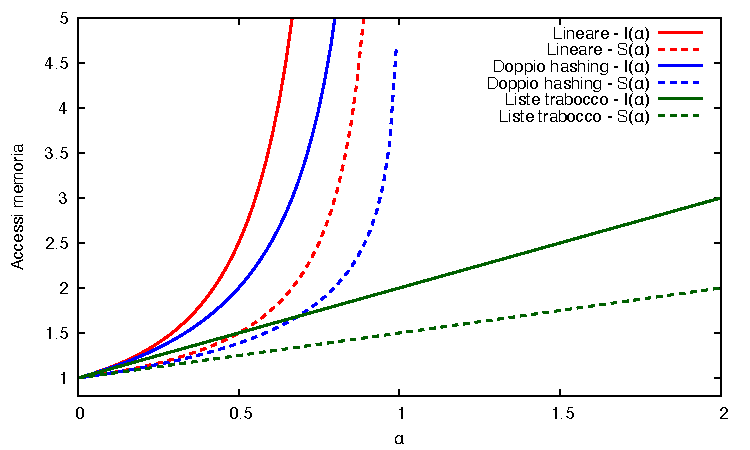
\includegraphics[width=\textwidth]{grafico.pdf}
	
\end{frame}

\begin{frame}{Ristrutturazione}

\BIL
\item Non è conveniente che $\alpha$ cresca troppo
	\BI
	\item In particolare con la scansione interna
	\item Ma vale anche per le liste di trabocco
	\EI
\item Sopra un soglia $t_\alpha$ prefissata (tipicamente $0.5$-$0.75$)
\BI
\item  Si alloca una nuova tabella di dimensione $2m$
\item Si reinseriscono tutte le chiavi presenti nella nuova tabella
\EI
\item Risultato
\BI
	\item Fattore di carico dimezzato (tipicamente $0.25$)
	\item Nessun elemento \textbf{deleted}
\EI
\item Costi
\BI
\item Costo $O(m)$ per la ristrutturazione nel caso pessimo
\item Costo ammortizzato costante (vedi dimostrazione per vettori)
\EI
\EIL

\end{frame}

\subsection{Reality check}

\begin{frame}[shrink=10]{Reality check}

{\renewcommand*{\arraystretch}{1.4}
\begin{tabular}{|P{2.5cm}|P{4.0cm}|P{0.6cm}|P{4.3cm}|}
\hline
\textbf{Linguaggio} & \textbf{Tecnica} & $t_\alpha$ & \textbf{Note} 
\\ \hline
%
Java 7\newline \texttt{HashMap} &
Liste di trabocco basate su \texttt{LinkedList} &
$0.75$ &
$O(n)$ nel caso pessimo \newline
Overhead: $16n + 4m$ byte
\\ \hline
%
Java 8\newline \texttt{HashMap} &
Liste di trabocco basate su RB Tree &
$0.75$ &
$O(\log n)$ nel caso pessimo \newline
Overhead: $48n + 4m$ byte
\\ \hline
C++ \newline \texttt{sparse\_hash} &
Ind. aperto, scansione quadratica & 
? &
Overhead: $2n$ bit
\\ \hline
C++ \newline \texttt{dense\_hash} &
Ind. aperto, scansione quadratica & 
$0.5$ &
$X$ byte per chiave-valore $\Rightarrow$ 2-3$X$ overhead
\\ \hline
C++ STL \newline \texttt{unordered\_map} &
Liste di trabocco basate su liste &
$1.00$ &
MurmurHash
\\ \hline
Python &
Indirizzam. aperto, scansione quadratica &
$0.66$ &
\\ \hline
\end{tabular}
}
\end{frame}





\begin{frame}[shrink=10]{Java \texttt{hashcode()}}
	
\vspace{-6pt}
\begin{myboxtitle}[Dalla documentazione di \texttt{java.lang.Object}]
The general contract of \texttt{hashCode()} is:
\begin{enumerate}
\item Whenever it is invoked on the same object more than once during an
execution of a Java application, \alert{\emph{the \texttt{hashCode()} method must consistently return
the same integer, provided no information used in equals comparisons on the
object is modified}}. This integer need not remain consistent from one execution
of an application to another execution of the same application.
\item \alert{\emph{If two objects are equal according to the \texttt{equals(Object)} method, then
calling the \texttt{hashCode()} method on each of the two objects must produce the same
integer result}}.
\item It is not required that if two objects are unequal according to the
\texttt{equals(Object)} method, then calling the \texttt{hashCode()} method on each of
the two objects must produce distinct integer results. However, \alert{\emph{the programmer
should be aware that producing distinct integer results for unequal objects may
improve the performance of hash tables}}.
\end{enumerate}
\end{myboxtitle}

\end{frame}


\begin{frame}{Java \texttt{hashcode()}}

\vspace{-6pt}
\BB{Se una classe non fa override di \texttt{equals()}:}
\BIL
\item Eredita i metodi
\texttt{equals()} e \texttt{hashCode()} così come definiti da \texttt{java.lang.Object}:
\BI
\item \texttt{x.equals(y)}  ritorna \textbf{true} se e solo se \texttt{x == y}
\item \texttt{x.hashCode()} converte l'indirizzo di memoria di \texttt{x} in un intero
\EI
\EIL

\BB{Se una classe fa ovveride di \texttt{equals()}:}
\BIL
\item "Always override hashCode when you override equals", in Bloch, Joshua (2008), Effective Java (2nd ed.)
\item Se non fate override, oggetti uguali finiscono in posizioni diverse
nella tabella hash
\EIL

\end{frame}

\begin{frame}{Java \texttt{hashcode()}}

\vspace{-6pt}
\BB{Esempio: \texttt{java.lang.String}}
\BIL
\item Override di \texttt{equals()} per controllare l’uguaglianza di stringhe
\item \texttt{hashCode()} in Java 1.0, Java 1.1
\BI
\item Utilizzati 16 caratteri della stringa per calcolare l’\texttt{hashCode()}
\item Problemi con la regola (3) - cattiva performance nelle tabelle
\EI
\item \texttt{hashCode()} in Java 1.2 e seguenti:
\[
  h(s) = \sum_{i=0}^{n-1} s[i] \cdot 31^{n-1-i}
\]
(utilizzando aritmetica \texttt{int})
\EIL

\end{frame}


\begin{frame}[fragile]{Java \texttt{hashcode()}}

\vspace{-6pt}
\BB{Cosa non fare}

\begin{lstlisting}[language=java]
public int hashCode()
{
  return 0;
}
\end{lstlisting}

\end{frame}

\section{Conclusioni}

\begin{frame}{Considerazioni finali}
	
\vspace{-6pt}
\BB{Problemi con hashing}
\BI
\item Scarsa "locality of reference" (cache miss)
\item Non è possibile ottenere le chiavi in ordine
\EI

\medskip
\BB{Hashing utilizzato in altre strutture dati}
\BI
\item Distributed Hash Table (DHT)
\item Bloom filters
\EI

\medskip
\BB{Oltre le tabelle hash}
\BI
\item Data deduplication
\item Protezioni dati con hash crittografici (MD5)
\EI

\end{frame}

	


\end{document}